
\section{Function composition and inverses}
In this chapter, we will look at composition of functions and inverse functions. You can use the normal arithmetic operations on functions like how you would to numbers:

\begin{example}{Arithmetic operations on functions}{}
  If \(x=2\) and \(f(x)=x^2+4\):
  \begin{equation*}
    f(x)+f(x) = 2^2+4+2^2+4=16 
  \end{equation*}
  \begin{equation*}
    \frac{f(x)}{2} = \frac{2^2+4}{2} = 4 
  \end{equation*}
\end{example}

What is more interesting, perhaps, is taking the \textit{output} of a function and use it as the \textit{input} to another function. You may also think of it as "piping" one function into another. This is called \textit{function composition}.


\begin{figure}[h]
  \centering

  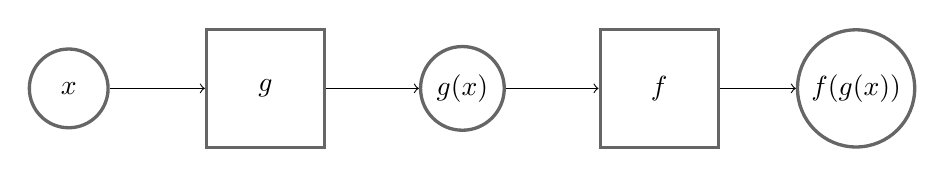
\begin{tikzpicture}[
      roundnode/.style={circle, draw=black!60, fill=white!5, very thick, minimum size=10mm},
      squarednode/.style={rectangle, draw=black!60, fill=white!5, very thick, minimum size=15mm},
      ]
      \node[roundnode] (x) {\(x\)};
      \node[squarednode] (maintopic) [right of=x, xshift=1.5cm] {\(g\)};
      \node[roundnode] (fx) [right of=maintopic, xshift=1.5cm] {\(g(x)\)};
      \node[squarednode] (gtopic) [right of=fx, xshift=1.5cm] {\(f\)};
      \node[roundnode] (final) [right of=gtopic, xshift=1.5cm] {\(f(g(x))\)};
      \draw[->] (maintopic.east) -- (fx.west);
      \draw[->] (x.east) -- (maintopic.west);
      \draw[->] (fx.east) -- (gtopic.west);
      \draw[->] (gtopic.east) -- (final.west);
  \end{tikzpicture}

  \caption{Visual representation of function composition. \sidenotemark}
\end{figure} 
\sidenotetext{\footnotesize \textit{Note that the rectangles are \\ functions and circles are values.}}

Another notation for composing functions together(which we will not really use except for this chapter) is as such:
\begin{equation*}
  f(g(x))=(f \circ g)(x) 
\end{equation*}

When you compose the same function \(n\)-times, the notation for it is\marginnote{\footnotesize \textit{However, this does not apply to trigonometric functions. \(\sin^2(x)\) is \(\sin(x) \times \sin(x)\) instead of \(\sin(\sin(x))\). Annoying mathematical notation strikes again. What is even better, is that \(f^{-1}(x)\) denotes the inverse of \(f\).}}:
\begin{equation*}
  f^n(x)=\underbrace{f(f(\ldots f(x)))}_{n-times} 
\end{equation*}

\begin{example}{Composing functions}{}
  Here are some examples of composing functions together:
  If \(x=3\) and \(f(x)=\pi x\), \(g(x)=\sin(x)+1\):
  \begin{equation}
    g(f(x))=\sin(\pi \times 3)+1=1 
  \end{equation}
  \begin{equation}
    f^3(x)=\pi^{3}x 
  \end{equation}
  There is nothing much here, really, just evaluate the function from the innermost function to the outermost.
\end{example}
\begin{theorem}{Composition of functions is associative}{}
  Given functions \(f:X \to Y\), \(g: Y \to Z\) and \(h: Z \to W\), prove that the composition of the three functions is \textit{associative}, in other words:
  \begin{equation*}
    h \circ (g \circ f(x)) = (h \circ g) \circ f(x)
  \end{equation*}
\end{theorem}
\begin{proof}{Composition of functions is associative}{}
  Let \(x \in X\), we have: 
  \begin{equation*}
    h \circ (g \circ f(x)) = h(g \circ f(x)) = h(g(f(x))) = h \circ g(f(x)) = (h \circ g)f(x)
  \end{equation*}
  This proves the associativity of function composition.
\end{proof}
\begin{remark}{}{}
  This is just a fun little exercise for the reader and ultimately is not that important to the entire book, just a good identity to keep in the back of your mind. 
\end{remark}

Next, we will delve into inverse functions. Let us start with one I believe you may have seen before, look at the following figure: 

\begin{figure}[h]
  \centering
  \begin{tikzpicture}[scale=1.8]
    \coordinate (a) at (0,0);
    \coordinate (b) at (4,0);
    \coordinate (c) at (4,2);
    \draw (a) -- (b)node[midway, below]{a} -- (c)node[midway,right]{b} -- (a)node[midway,left, above]{c}; % Triangle.
    \draw (a) node[anchor=east,align=center] {B};
    \draw (b) node[anchor=west,align=center] {C};
    \draw (c) node[anchor=south]{A};
    \MarkRightAngle{a}{b}{c}; 
  \end{tikzpicture}
  \caption{Figure of right triangle ABC.}
\end{figure}

If I ask you what is \(\arcsin(B)\), you may say it is \(\frac{b}{c}\). But, what is \(\arcsin(\sin(B))\), well, that is just \(B\), isn't it. Hence, the \(\arcsin\) sort of "cancels" the \(\sin\). We call \(\arcsin\) the \textit{inverse function} or just inverse of \(\sin\).\sidenote{\footnotesize \textit{We will use \(\arcsin\) as the inverse of \(\sin\) instead of \(\sin^{-1}\) as it is clearer.}} Generally, given a function \(f: X \to Y\), \(f^{-1}\) denotes the inverse function that satisfies:
\begin{equation}
  f \circ f^{-1}(y) = y, y \in Y \text{\, and \,} f^{-1} \circ f(x) = x, x \in X
\end{equation}

\begin{note}{Cancelling functions and their "inverse"}{}
  One common misconception is that \(f(f^{-1}(x))=f^{-1}(f(x))\) for any function. While this is technically true, you may apply this fact wrongly. For example, take the following function:
  \begin{equation*}
    f(x)=\sin(x), f^{-1}: \{y: -1 \leq y \leq 1 \} \to \mathbb{R}
  \end{equation*}
  This looks deceptively simple, when asked to evaluate \(f^{-1}(f(\pi))\), it is \(\pi\) (You may want to verify it yourself). But what is \(f(f^{-1}(\pi))\)? Well, according to our definition of \(f\), \(f^{-1}(\pi)\) is simply not defined. In actuality, to find \(f^{-1}(\pi)\), we need complex numbers, which is not allowed in the definition. Hence, you must be extra careful when you are dealing with function inverses and pay attention to the domain and range.
\end{note}

To find the inverse function of a function \(f\), we have to find the function that maps the outputs of the \(f\) back to its inputs. To solve algebraically, we set \(f(x)\) for some arbitrary \(x\) to \(y\), and make \(x\) the subject of the equation.
\begin{example}{Finding the inverse of a function}{}
  Given that \(f(x)=\frac{x+7}{3}\):
  \begin{align*}
    f(x)&=y \\
    \frac{x+7}{3}&=y \\
    x+7&=3y \\
    x&=3y-7
  \end{align*}
  Hence, the inverse function is \(f^{-1}(y)=3y-7\).
\end{example}
\begin{example}{Common inverse functions}{}
  Some common examples of inverse functions:
  \begin{enumerate}
    \item{Trigonometry: \begin{align*}
        \arcsin && \arccos && \arctan && \dots 
    \end{align*} } 
  \item{Logarithms (Inverses of exponential functions): \begin{align*}
      \ln && \log_{b} 
  \end{align*} }
  \end{enumerate}
\end{example}
\hrule
\begin{problem}

  Given \(f(x)=\frac{x^2+3}{2}\) and \(g(x)=\tan(x)+1\), evaluate:
  \begin{enumerate}[label=\alph*)]
    \item{\(f(g(\frac{\pi}{4}))\)}
    \item{\(f^{3}(1)\)}
    \item{\(f(g(\arcsin(0)))\)}
  \end{enumerate}

\end{problem}
\begin{problem}

  Given that \(h(x)=(x-7)^2, \, x \geq 7\), find the inverse of \(h\).
  Hence, evaluate:
  \begin{enumerate}[label=\alph*)]
    \item{\(h^{-1}(1)\)}
    \item{\(h(h^{-1}(69))\) \textit{As Peter Lorre would have said it, "Do it ze kveek vay, Johnny".}}
  \end{enumerate}
\end{problem}


\begin{problem}[1]
  The \textit{dirac delta function} is defined as 
  \begin{equation}
    \delta(x)=\begin{cases}
      \infty & x=0 \\
      0 & \textit{otherwise}
    \end{cases}
  \end{equation}


  It also has an area of 1 "underneath" it.

  \begin{enumerate}[label=\alph*)]
    \item{Show that \(f(x)\delta(x-a)=f(a)\delta(x-a)\).}
    \item{Hence, simplify \((3x^2-2x-1)\delta(x-3)\).}
  \end{enumerate}
  \label{diracpb}
\end{problem}
\begin{problem}[1]
  Given that the function \(f(x)\) is defined as \(f(x)>f(x-1)+f(x-2)\), and when \(x<3\), \(f(x)=x\), show that \(f(20)>1000\). \textit{(Adapted from the 2024 Chinese College Entrance Examination)} 
\end{problem} 
%
% \begin{enumerate}
%   \item{
%       \begin{enumerate}
%         \item{\(\frac{7}{2}\)}
%         \item{\(\frac{61}{8}\)}
%         \item{2}
%       \end{enumerate}
%     } 
%   \item{\(h^{-1}(y)=\sqrt{y}+7\)}
%   \item{
%       \begin{enumerate}
%         \item{8}
%         \item{69 (Inverse function and the original function "cancels".)}
%       \end{enumerate}
%     }
% \end{enumerate} 
